\documentclass[border=8pt]{standalone}
\usepackage{tikz}
\usetikzlibrary{arrows.meta,positioning,calc,backgrounds}
\definecolor{cjob}{RGB}{72,116,158}
\definecolor{cmac}{RGB}{86,156,104}
\definecolor{chl}{RGB}{214,133,55}
\definecolor{cchg}{RGB}{198,86,76}
\begin{document}
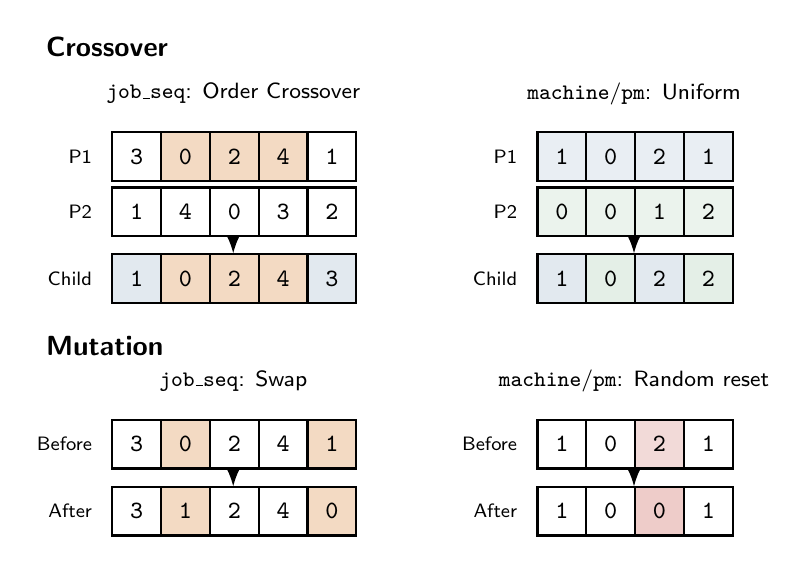
\begin{tikzpicture}[
  font=\sffamily\small,>=Latex,
  cell/.style={draw,thick,minimum size=0.62cm,inner sep=0pt,anchor=west,font=\ttfamily\small},
  rlab/.style={anchor=east,font=\sffamily\scriptsize},
  hdr/.style={anchor=center,font=\sffamily\footnotesize},
  ttl/.style={anchor=west,font=\sffamily\bfseries},
  arrow/.style={->,thick}
]
% ---- titles ----
\node[ttl] at (-0.95,1.95) {Crossover};
\node[ttl] at (-0.95,-1.85) {Mutation};

% ---- sub headers ----
\node[hdr] at (1.55,1.35) {\texttt{job\_seq}: Order Crossover};
\node[hdr] at (6.64,1.35) {\texttt{machine}/\texttt{pm}: Uniform};
\node[hdr] at (1.55,-2.30) {\texttt{job\_seq}: Swap};
\node[hdr] at (6.64,-2.30) {\texttt{machine}/\texttt{pm}: Random reset};

% ================= OX =================
\foreach \v [count=\i from 0] in {3,0,2,4,1} {\node[cell] (oxp1-\i) at ({0.62*\i},0.55) {\v};}
\foreach \v [count=\i from 0] in {1,4,0,3,2} {\node[cell] (oxp2-\i) at ({0.62*\i},-0.15) {\v};}
\foreach \v [count=\i from 0] in {1,0,2,4,3} {\node[cell] (oxch-\i) at ({0.62*\i},-1.00) {\v};}
\node[rlab] at (-0.12,0.55) {P1};
\node[rlab] at (-0.12,-0.15) {P2};
\node[rlab] at (-0.12,-1.00) {Child};
\draw[arrow] (1.55,-0.47) -- (1.55,-0.68);

% ================= Uniform =================
\foreach \v [count=\i from 0] in {1,0,2,1} {\node[cell] (ucp1-\i) at ({5.4+0.62*\i},0.55) {\v};}
\foreach \v [count=\i from 0] in {0,0,1,2} {\node[cell] (ucp2-\i) at ({5.4+0.62*\i},-0.15) {\v};}
\foreach \v [count=\i from 0] in {1,0,2,2} {\node[cell] (ucch-\i) at ({5.4+0.62*\i},-1.00) {\v};}
\node[rlab] at (5.28,0.55) {P1};
\node[rlab] at (5.28,-0.15) {P2};
\node[rlab] at (5.28,-1.00) {Child};
\draw[arrow] (6.64,-0.47) -- (6.64,-0.68);

% ================= Swap =================
\foreach \v [count=\i from 0] in {3,0,2,4,1} {\node[cell] (swb-\i) at ({0.62*\i},-3.10) {\v};}
\foreach \v [count=\i from 0] in {3,1,2,4,0} {\node[cell] (swa-\i) at ({0.62*\i},-3.95) {\v};}
\node[rlab] at (-0.12,-3.10) {Before};
\node[rlab] at (-0.12,-3.95) {After};
\draw[arrow] (1.55,-3.42) -- (1.55,-3.64);

% ================= Reset =================
\foreach \v [count=\i from 0] in {1,0,2,1} {\node[cell] (rsb-\i) at ({5.4+0.62*\i},-3.10) {\v};}
\foreach \v [count=\i from 0] in {1,0,0,1} {\node[cell] (rsa-\i) at ({5.4+0.62*\i},-3.95) {\v};}
\node[rlab] at (5.28,-3.10) {Before};
\node[rlab] at (5.28,-3.95) {After};
\draw[arrow] (6.64,-3.42) -- (6.64,-3.64);

% ================= highlights (background) =================
\begin{scope}[on background layer]
  \fill[chl!30] (oxp1-1.north west) rectangle (oxp1-3.south east);
  \fill[chl!30] (oxch-1.north west) rectangle (oxch-3.south east);
  \fill[cjob!16] (oxch-0.north west) rectangle (oxch-0.south east);
  \fill[cjob!16] (oxch-4.north west) rectangle (oxch-4.south east);
  \fill[cjob!12] (ucp1-0.north west) rectangle (ucp1-3.south east);
  \fill[cmac!12] (ucp2-0.north west) rectangle (ucp2-3.south east);
  \fill[cjob!16] (ucch-0.north west) rectangle (ucch-0.south east);
  \fill[cmac!16] (ucch-1.north west) rectangle (ucch-1.south east);
  \fill[cjob!16] (ucch-2.north west) rectangle (ucch-2.south east);
  \fill[cmac!16] (ucch-3.north west) rectangle (ucch-3.south east);
  \fill[chl!30] (swb-1.north west) rectangle (swb-1.south east);
  \fill[chl!30] (swb-4.north west) rectangle (swb-4.south east);
  \fill[chl!30] (swa-1.north west) rectangle (swa-1.south east);
  \fill[chl!30] (swa-4.north west) rectangle (swa-4.south east);
  \fill[cchg!22] (rsb-2.north west) rectangle (rsb-2.south east);
  \fill[cchg!30] (rsa-2.north west) rectangle (rsa-2.south east);
\end{scope}
\end{tikzpicture}
\end{document}
